\documentclass[a4paper]{article}
\usepackage[colorlinks=True, linkcolor=blue, urlcolor=blue]{hyperref}
\usepackage[]{geometry}
\usepackage{amsmath}
\usepackage{amssymb}
\usepackage{graphicx}
\usepackage{listings}
\usepackage{color}

\definecolor{string}{RGB}{170, 55, 241}
\definecolor{comments}{RGB}{6, 186, 72}
\lstset{language=Matlab, numbers=left,
	breaklines=true, commentstyle=\color{comments},
	stringstyle=\color{string}, keywordstyle=\color{blue},
	emph=[1]{ylim,xlim}, emphstyle=[1]\color{blue}}

\title{Project Elective\\{\Large{Course report} }}
\author{Shubhayu Das(IMT2018523)}

\begin{document}
	\maketitle
	\tableofcontents

	\pagebreak

	\section{Problem Statement}
		The human knee joint is crucial to perform locomotion. It can be modelled as a hinge joint, with adaptions to bear a large body weight. The knee joint has evolved to absorb shocks, while jumping for instance. Inability to move the knee effectively puts an end to free locomotion in humans. Heart stroke in humans can cause inabiltiy to move their lower limbs.\\

		The goal of this project is to design a robotic device, which will help in rehabilitation. The device must be easy to use, with all necessary safety precautions implemented in software. The system must be able to accomodate additional sensors in the future, which will enable monitoring the patient's neural activity in the lower limb in question.\\

		\textit{This report, along with the simulation files and other presentations can be found in \href{https://github.com/Shubhayu-Das/PE_6th_sem}{this GitHub repository}. The content of repository will be updated over time, with all that I learnt. This report contains a high level summary of all aspects of the project.}

	\section{Approach}
		The chosen approach is to position and attach a motor, whose axis of rotation aligns with that of the knee joint. The basis of selection of the motor's parameters: the mass and the torque, was decided on basis of a simulation performed using the Webots platform.\\

		The motor needs to be capable of assisting the rotational movement of the knee joint. In a majority of the target exercises, this involves lifting the leg(the shin and the foot), along with the lower part of the harness. For an assumed peak angular velocity of the knee joint, we can work out the peak and continuous torque requirements. Being a widely researched field, journal [1] was referred to, which summarizes the approaches of a variety of research teams.\\

	\pagebreak
	\section{Simulation}
		The simulation was performed using the Webots R2021a stable release on Windows 10. The setup can be seen in the following image:

		\begin{center}
			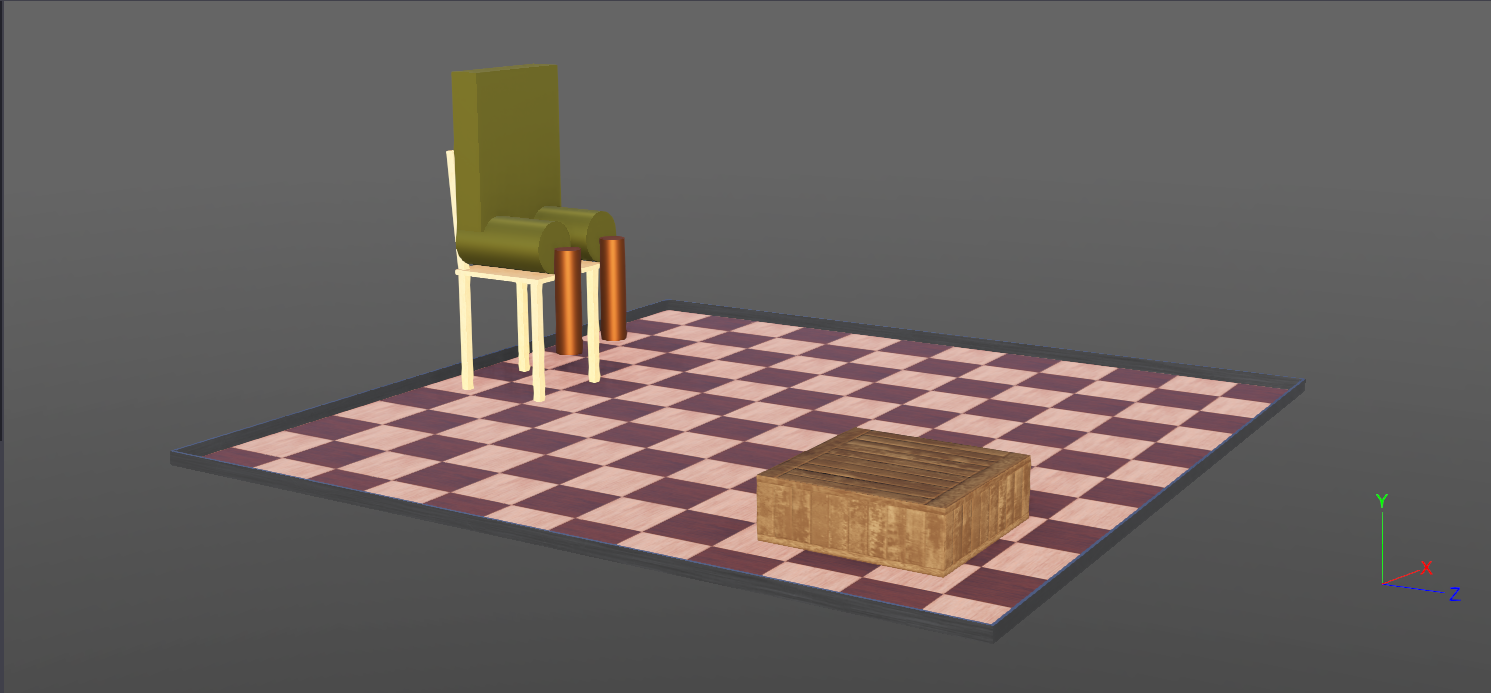
\includegraphics[width=\linewidth]{"../images/sideview.png"}
			\title{An image of the simulation setup. The position of the box indicates the "right" side, wrt to the humanoid robot.}
		\end{center}

		The simulation was performed using the following parameters:
		\begin{itemize}
			\item Mass of the torso+thighs(in yellow): 50kg
			\item Mass of each shin, along with assumed harness weight(cylinder down from the knee joint): 10kg
			\item Peak angular velocity: nearly $\pi$ rad/s
			\item Simulation timestep: 32ms
		\end{itemize}

		The positions of each of the mobile joints are monitored and logged after every 8 simulation updates in a csv file. The relevant parameters are then plotted separately to visualize the torque requirements, as a function of the angular position. This plot is show in the plot on the next page.

		\begin{center}
			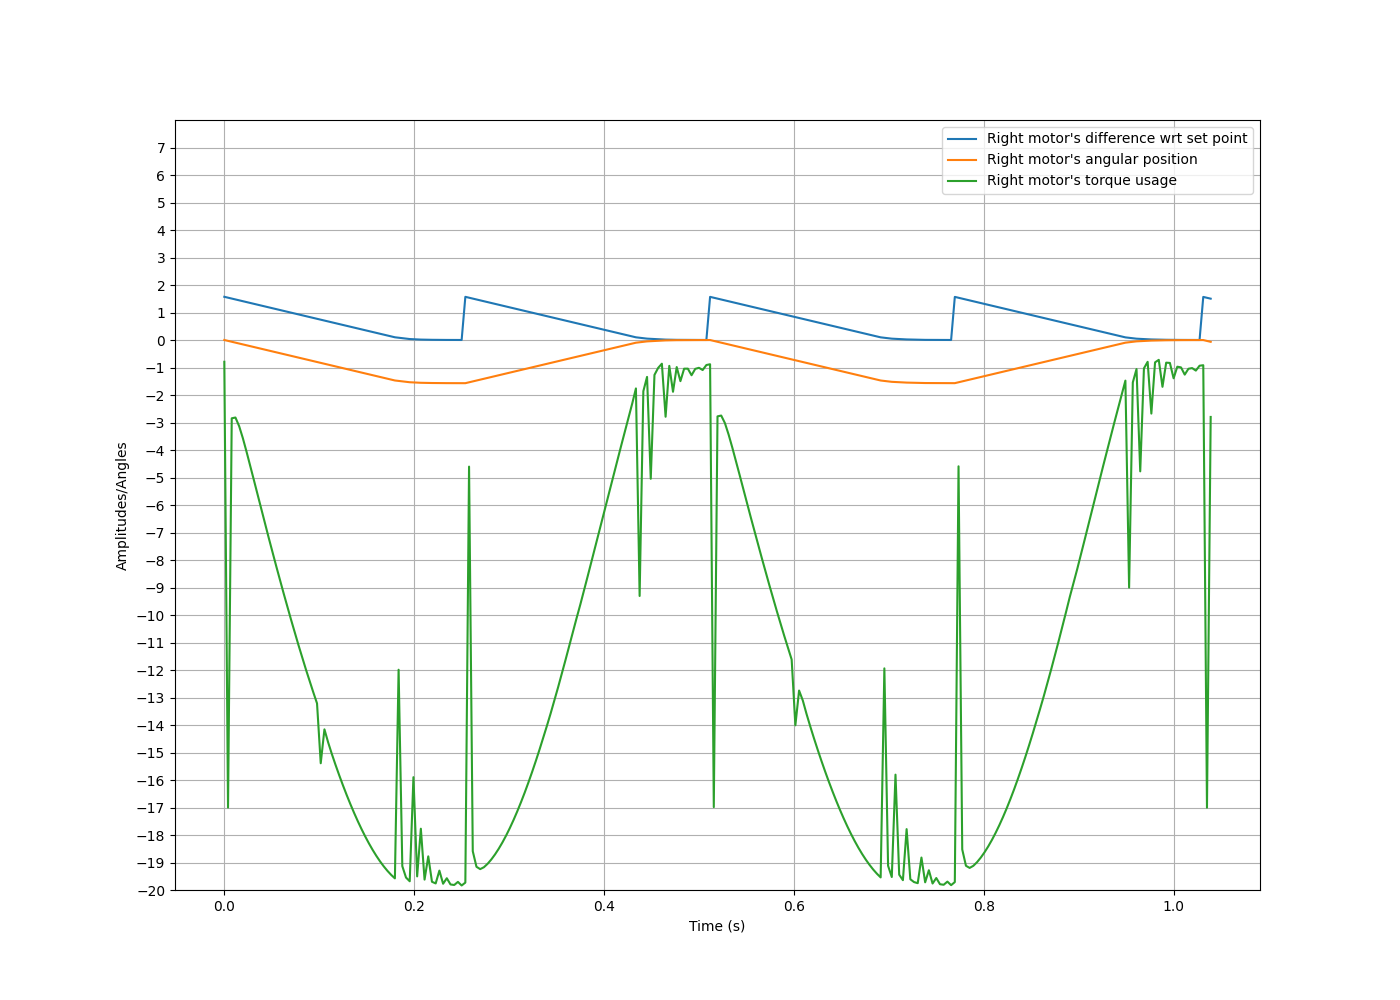
\includegraphics[width=\linewidth]{"../images/sim_results.png"}
			\title{Plot of the data output by the simulation. The blue line shows the angular difference between the setpoint and the current position in radians. The orange line shows the current angular position in radians. The green line shows the torque output from the motor at the "right" knee in Nm.}
		\end{center}

		Note that the PID control is the default controller in Webots. Further tuning can help smooth out the spikes in the torque plots. These spikes bring out the limitations of simulations. Further, the torque values are negative due to the frame of reference of the knee joint.\\

		A 1:1 CAD model of the motor(T-Motors AK80-6) was designed using AutoDesk Fusion 360 as well. This can be further utilized to design the harness and decide on the position of the motor(s).

		\begin{center}
			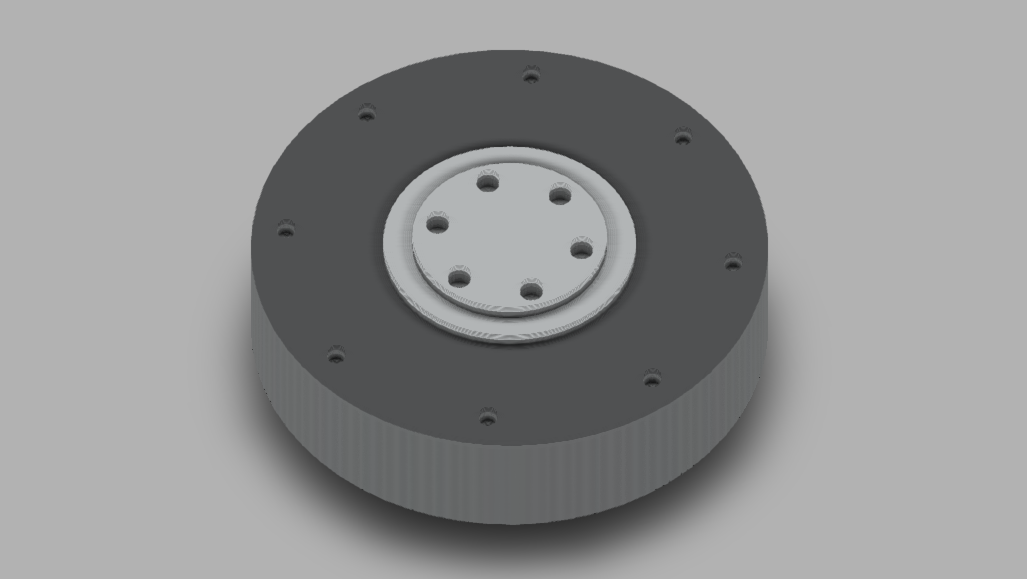
\includegraphics[width=\linewidth]{"../images/AK80-6 CAD.png"}
			\title{An image of the 3D CAD model. The model can be found in the GitHub repository, or alternatively can be downloaded from this \href{https://a360.co/3pVPdYg}{Autodesk online link}.}
		\end{center}

	\section{Literature Review}
		Several papers were referred to, to verify and confirm the validity of the torque simulations. A variety of papers report extremely high torque requirements($\ge100Nm$), which is unrealistic. Kong et. al. [2, figure 3], report the torque needed, as a function of the angular velocity. Their modelling is to \textit{fully} support a walking human, which is out of scope. However, the design can be adapted to accomodate for this posibility as well.

	\section{Selected hardware}
		Using the results from the simulations and the literature surveys, it was decided to choose a motor with atleast 20Nm of torque, going upto 40Nm. To achieve such high torques, gearboxes are a must, to keep things relatively inexpensive. Brushless DC motors(BLDC motors) are the perfect candidates for the task. The other factor to consider is the weight of the motor(combined with the gearbox and the interface with the harness).\\

		The gearbox must be back-drivable, to allow the wearer to exert forces, depending on their muscle strength(and the motor's torque limit, set in software). Additionally, the gearbox must be capable of tolerating stress perpendicular to its axis. BLDC motors are typically high RPM, low torque motors. So a moderate reduction ratio(~30:1) is needed, which must be compact and resistant to wear. If possible, the backlash error must be kept at a bare minimum. This comes down to the precise design of the gears, along with the chosen configuration.\\

		\subsection{Motors}
			I chose one T-Motor CubeMars AK80-6 100KV, which capable of delivering a continuous torque of 6Nm at upto 400RPM, when operated at 24V. This is an outer runner BLDC motor, with an inbuilt 6:1 reduction planetary gear system. I have planned to additionally add an external 6:1 reduction gearbox(possibly planetary) to meet the torque requirements, along with the rotational velocity.\\

			Given that this actuator is a pretty expensive solution, I have further chosen a T-Motor CubeMars RI50 KV100 BLDC inner runner motor. Note that this is the bare motor stator, along with the permanent magnets only. This product is one order of magnitude cheaper, but needs a custom design for the gearbox, body and motor driver. Inspite of this, the overall product is estimated to cheaper, with a significantly higher design time. This motor is capable of delivering a continuous torque of 0.6Nm at upto 3000RPM. So with an overall reduction of 36:1, we can expect an effective torque of around 15-20Nm. This should ideally be enough, given that we are only trying to assist the patient.\\

			Additional information about the actuators can be found in the official T-Motor website. I referred to Skyentific's YouTube channel to get an overview on how to setup and use these motors. The link is available in the references section.

		\subsection{Gear box}
			The external gearboxes are intended to be planetary gearboxes, with fixed ring gears. Planetary gearboxes are relatively easy to prototype using 3D printed parts. Cycloidal gearboxes are another possibility, but they are hard to work with while 3D printing. They further need a lot of bearings and 2 cycloidal discs to ensure proper operations. Strain wave gears are out of question too, due to durability problems of 3D printed components. They are not back-drivable either, and might slip too. The target reduction ratio is 6:1 for any gearbox.\\

			I referred to James Brunton's YouTube channel to learn about these, along with Skyentific's YouTube channel. Both are linked in the description below.

		\subsection{Motor driver}
			The AK80-6 motor includes a MIT Mini Cheetah actuator, designed by Ben G. Katz at MIT, USA. This is a typical 3 phase 3 phase H-bridge BLDC motor driver design. He utilized Texas Instruments DRV8323R 3 phase gate driver, along with suitable MOSFETS from Toshiba electronics(TPH2R506PL). THe driver is controlled using a ARM Cortex M4 MCU from STMicroelectronics(STM32F446RETx). The general circuit and PCB design are similar to the reference design on TI's webpage for the motor driver, under "Technical documentation"[3].\\

			The motor driver is accompanied with an AS5147P, 14 bit magnetic encoder. This is needed for the closed loop control of the BLDC motors, as described in the next section. I referred to MATLAB's YouTube videos on BLDC motor control, along with TI's application notes and Skyentific's demo video on YouTube. All of them are linked in the references section.

		\subsection{Master controller}
			I plan to use an ARM Cortex M4 microcontroller from STM(STM32F407VGT) to send commands to the individual motor drivers, which have their own MCUs. This ARM MCU is seriously overkill, but it is the only MCU available at hand, with all the requisite features(CAN support, lots of memory, large amount of IO, high clock speed). Any non-ARM MCU with the same features should work equally well.\\

			The MCU will perform data logging(either internally, or over USB, to a computer). Additionally, an ESP32 can be added to enable Wi-Fi connectivity to the setup. The possibility of just using an ESP32 with RTOS needs to be explored as well. I referred to the Mutex Embedded YouTube channel and Phil's Lab on YouTube learn how to work with STM MCUs. Both are linked in the references section.

	\section{Control Software}
		Good hardware is only half of the story. Proper BLDC control is impossible without proper driver control software. The MIT Mini Cheetah driver implements Field Oriented Control(FOC), using position feedback from the encoder, and torque feedback from the low-side current sense resistors. The DRV8323R motor driver facilitates the torque feedback by providing internal gain amplifiers and buffers. In this project, we directly utilize Ben Katz's driver code(Github source),as we are using his drivers. Some parameters like the PID gains, reduction ratios etc have to be calibrated depending on the actual hardware being used.\\

		Note that the MIT Mini Cheetah driver uses CAN communication protocol, which a good industry standard. The MCUs chosen must be capable of communicating using CAN (either directly, or using a CAN shield).\\

		The exact working principle of FOC can span several books. I have summarized my understanding in the source Github repository. The content of the repository are subject to change, during the active duration of this project.

	\section{Pending work}
		The COVID-19 pandemic prevented me from staying and working in the campus. As a result, none of the concepts mentioned above have actually beem tested. The motors, along with the requisite power supply are available in campus.\\

		 I collected two STM32F4 Discovery boards from the CEEMS lab, to try and learn how to work with their ecosystem. I successfully tested a lot of other features, but my attempts to setup CAN communication between the two boards failed, due to lack of proper transceivers. I procured the requisite tranceivers, but couldn't use them due to lack of soldering equipment at home. These components will be duly returned to the labs whenever possible.\\

		 The position and torque control FOC algorithms need to be tested and tweaked as per need. The MIT Mini Cheetah controller uses CAN bus communication to transmit the set point, PI control variables($K_p, K_i$) and the torque. These need to be handled by the master controller, which will compute the trajectory of motion, along with the torque calculations. Safety features such as emergency position holding need to be implemented in software.

	\vspace*{1cm}
	\section{References}
		I found a plethora of good references videos on YouTube, along with technical documents from Texas Instruments, STMicroelectronics and MATLAB. These were excellent sources of information, which taught me the basics of all of the content mentioned above. The links are all valid and functional at the time of writing this report. They are subject to change in the future.\\

		\noindent\href{https://github.com/Shubhayu-Das/PE_6th_sem}{Link to GitHub repository for this project}. Note that I am \textit{not} adding a lot of files that are not open sourced/licensed to be freely distributed. Most of them are linked below.\\

		Here are the papers and technical documents:
		\begin{enumerate}
			\item\href{https://doi.org/10.1016/j.robot.2019.103394}{L. Zhang, G. Liu, B. Han et al., Assistive devices of human knee joint: A
				review, Robotics and Autonomous Systems (2019), doi:
				https://doi.org/10.1016/j.robot.2019.103394}
			\item \href{https://ieeexplore.ieee.org/document/5509227}{Kyoungchul Kong, Joonbum Bae,Masayoshi Tomizuka, A Compact Rotary Series Elastic Actuator for Knee Joint Assistive System}
			\item \href{https://www.ti.com/product/DRV8323R#tech-docs}{TI DRV8323R product page}
		\end{enumerate}

		Here are some of the YouTube playlists/content creators who helped me learn a lot about each component of the entire flow:
		\begin{itemize}
			\item \href{https://in.mathworks.com/solutions/power-electronics-control/bldc-motor-control.html}{MATLAB's BLDC Motor Control webpage, contains links to YouTube playlist.}
			\item \begin{itemize}
				\item \href{https://www.youtube.com/c/Skyentific/videos}{Skyentific's YouTube channel}
				\item \href{https://www.youtube.com/watch?v=WKRLlthr9kY}{Skyentific's demo on how to build the MIT Mini Cheetah motor driver}
				\item \href{https://www.youtube.com/watch?v=HzY9vzgPZkA}{Skyentific's review of the T-Motor A80-6 actuator}
				\item \href{https://www.youtube.com/watch?v=Wb1gsJ4K4pM}{Skyentific's comparison of 3 different BLDC FOC motor drivers}
			\end{itemize}
			\item \href{https://www.youtube.com/watch?v=Mhxz2Bj2RXA}{Teardown of the MIT Mini Cheetah actuator.} This is a very good video to watch, to understand the internal structure of BLDC motors.
			\item \href{https://www.youtube.com/watch?v=Fb6HQNZ4PzQ}{Demo of the MIT Mini Cheetah motor, with its motor driver.}
			\item \href{https://www.youtube.com/playlist?list=PLQFVvDcd2teniWVcMVeDBWkRVxNjirC6K}{TI's videos on "Teaching Old Motors new tricks", compiled into a single playlist by Yamming Luo. The original videos are available on TI's YouTube channel}
			\item \href {https://www.youtube.com/watch?v=uJvPwxa5n00&list=PLfExI9i0v1sn_lQjCFJHrDSpvZ8F2CpkA}{Mutex Embedded - Education YouTube channel's tutorial playlist on the STM32F407VGT. The IDE in use has changed ever since.}
			\item \href{https://www.youtube.com/playlist?list=PLXSyc11qLa1a4Tqbz228dPZfMrs-KRpzA}{Phil's Lab - YouTube playlist on working with STM32 boards using the STM32CubeMXIDE. This is among the latest series, as of May 2021}
			\item \href{https://www.youtube.com/c/jamesbruton/videos}{James Brunton's YouTube channel with many videos on gearboxes, with open source design files, meant to be 3D printed}
			\item \href{https://www.youtube.com/c/stmicroelectronics/playlists}{STMicroelectronics YouTube channel with hundreds of videos on working with their MCUs, deploying ML/AI algorithms etc.} They have videos on motor control too, for their portfolio of motor drivers and MOSFETs.
		\end{itemize}

		Here are some Github repositories which are essential for this project to work:
		\begin{itemize}
			\item \href{https://github.com/bgkatz/motorcontrol}{Ben Katz's updated motor control code, re-written to work with the STM32CubeIDE}
			\item \href{https://github.com/bgkatz/3phase_integrated}{Ben Katz's original motor driver code, used in the MIT Mini Cheetah project.}
			\item \href{https://github.com/mjbots/moteus}{MJ Bots alternative firmware for the MIT Mini Cheetah motor driver.} Need to check for compatibility, as they have redesigned the hardware slightly. Their KiCAD PCB schematics are available in the repository too.
			\item \href{https://github.com/odriverobotics/ODrive}{O-Drive's repository containing all their project files}. They are a very popular open-source motor driver project, with very good controllers. The circuit design is similar to that of MJ Bots/MIT Mini Cheetah. The firmware is very different.
			\item \href{https://github.com/G-Levine/OpenTorque-Actuator}{Gabrael Levine's extensive design for a planetary reliable gearbox.} This can be used as a reference for our design.
			\item \href{https://github.com/STMicroelectronics/STM32CubeF4}{STM's firmware packages for STM32F4 line of MCUs.} Contains good examples, and is downloaded and used by STM32CubeIDE.
		\end{itemize}
\end{document}
